\chapter{Program Counter Incrementer and Mux}

As mentioned in the last lab, the program counter is a register that is one word in length.  It holds the address in memory of the next instruction to be fetched and executed.  There are several ways that the program counter is updated:  
\begin{enumerate}
	\item If the program does not branch (via an if statement, while loop, etc), then the program counter should advance to the next address (by adding 4 to the current PC) each clock cycle.
	\item If the conditions of a conditional branch are met, then the program counter should be updated with the branch destination address.
	\item If an unconditional branch or jump occurs, then the program counter should be updated with the branch destination address.
	\item If an interrupt or error occurs, then the program counter should be updated with the interrupt or error handler address.
\end{enumerate}
The instructions will be fetched in sequential order the majority of the time.

\section{Adder}

We will build a program counter incrementer by making a simple adder.  Later in our computer we will need another adder, so we will re-use this code.  Therefore, the adder code should be stored in ARM-Lab/code/0\_common because it will be used in multiple stages.  When used as the program counter, we will pass it a 4 because each instruction is 32-bits long (even though it is a 64-bit computer) and we want to increment to the next instruction in memory.  Most machines are byte addressable, because one ASCII character (a char in c/c++) is a byte.  For a machine with 32-bit instructions like we are using, that would mean that each instruction would be 4 bytes later in memory ($32/8=4$ bytes).  Therefore, we will be adding 4 to the program counter each time we want to increment the program counter.

An adder is very simple in Verilog.  There are two inputs (the two numbers to be added) and one output (the result).   All the ports are size `WORD because they hold 64-bit integers.  

In this lab you will make your own adder module.  Your adder module should be called 'adder' and should have inputs of \verb1a_in1 and \verb1b_in1.  The output should be \verb1add_out1.  HINT: this should be very easy.  Verilog is a Hardware Description Language, so use Verilog to describe what you want to do.  Don't make it complicated.  The adder code should be stored in ARM-Lab/code/0\_common/adder.v.  You will need to create this file.

\section{Adder Test Bench}
I have provided an incomplete test bench for the adder.  While I put most of the infrastructure in place, you will need to fill in the following details.  I labeled these spots with comments that start with TODO so that you can see where you need to do your work.
\begin{enumerate}
	\item Create an instance of the adder module
	\item Fill in the details of each test case so that your simulation results and test log match the results shown in Figure~\ref{fig:addertestsimulationresults} and Figure~\ref{fig:addertestlog}.  Pay careful attention to detail to make sure your results are identical to these figures.  This includes making sure that the timing matches.
\end{enumerate}

\begin{figure}
	\caption{Adder Test Simulation Results}\label{fig:addertestsimulationresults}
	\begin{center}
		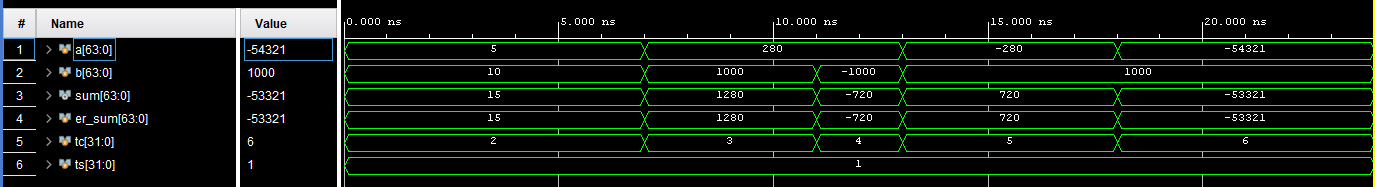
\includegraphics[width=4.75in]{../images/adder_test_simulation_results.png}
	\end{center}
\end{figure}

\begin{figure}
	\caption{Adder Test Log}\label{fig:addertestlog}
	\begin{center}
		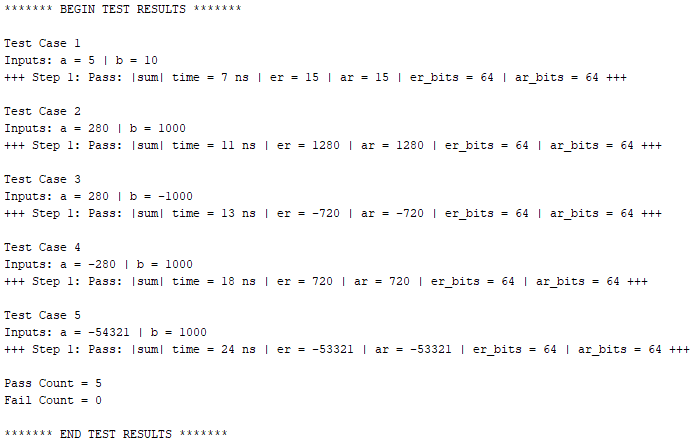
\includegraphics[width=4.75in]{../images/adder_test_log.png}
	\end{center}
\end{figure}

\section{Input Selection via Mux}

We will also need to be able to choose between normal advancing (sequential stepping) and branching (loops, if statements, etc.).  We will use a multiplexor (mux) to do this.  A mux is a simple device that connects one of the inputs to the output based on how the control bit is set.  If the control bit is 0 then input a is connected to the output, and if the selector is 1 then input b is connected to the output.  The heading and port list is provided for you in Listing~\ref{code:mux}.  You just need to fill in the body to make it operate like a mux.  

One interesting addition in this block of code is the addition of a size parameter.  Parameters allow you to pass a value into a module, making the module more flexible and reusable.  In the mux code, the parameter is specificed by \#(parameter SIZE=8).  Parameters are constants, so they cannot be explicitly changed within the module.  Rather, they are specified when an instance of this module is created.  In the provided mux\_test.sv, the mux module is instantiated by: mux \#(`WORD) UUT\_64.  Note that `WORD is a macro (from definitions.vh) that defines another name for the value 64.  So the test bench passes in a parameter value of 64, and the mux module uses 64 anywhere the term SIZE is used.  If no parameter is specified when the instance is created, then the parameter will be assigned the default value.  $SIZE=8$ defines the default value for the SIZE parameter in this module.

Note parameters are constants and cannot be changed later in the module.  In this lab, we are using parameters to set the number of wires that compose the inputs and output.  In our lab project, we will need some muxes to switch entire words (64 bits) like this one, but later we will also need to switch register addresses (5 bits).  Rather than write two muxes, we will make one and then use the parameter to change the size when they are declared.  The mux code should be stored in ARM-Lab/code/0\_common/mux.v.

The provided testbench instantiates both a 64 bit mux and a 5-bit mux so that two different mux sizes can be tested, ensuring that the mux works now and will work when we use it later in the semester.

\Verilog{Verilog code to make a mux.}{code:mux}{../code/0_common/mux.v}

\section{Your Assignment}

You are to:
\begin{enumerate}
\item Create an adder module.
\item Update adder\_test.sv as described above.	
\item Fill in the body of the mux module in mux.v.
\item Use the provided mux\_test.sv to verify that the mux works properly.  Note that you cannot/should not make any changes to the test bench.  The correct results are already in the test bench.	
\item Produce a landscape mode PDF called Lab2\_lastname.pdf that includes (in this order):
\begin{enumerate}
	\item Your name and the lab number.
	\item A snip of the Simulation Results for the adder\_test.  Make sure to show all values in decimal form and don't cut off the signal names on the left.  
	\item The adder\_test results copied and pasted from the Tcl Console.  The results should show the entire log from BEGIN TEST RESULTS to END TEST RESULTS.
	\item A snip of the Simulation Results for the mux\_test.  Make sure to show all values in decimal form and don't cut off the signal names on the left.  
	\item The mux\_test results copied and pasted from the Tcl Console.  The results should show the entire log from BEGIN TEST RESULTS to END TEST RESULTS.
\end{enumerate}
\item Upload Lab2\_lastname.pdf file to Canvas.
\item Zip up your ARM-Lab directory and submit it on Canvas as well.  Please make sure that you give me the ARM-Lab directory rather than the ARM-Project directory.  I do not want the project files in the ARM-Project directory.  Before you submit your zip file, extract the file and make sure that the top-level directory is called ARM-Lab and that the lower level directories like code, manual, etc are directly beneath ARM-Lab in the directory structure.  I will extract your zip file and run your code against my correct testbench to verify that your code and testbench work correctly, and it is critical that everyone's directory structure is consistent.
\end{enumerate} 